% Ekstremumspunkter
%
\begin{frame}
\frametitle{Hjørner}
\begin{itemize}
\item Ekstremumspunkter
\begin{itemize}
\item Ikke konveks kombination
\end{itemize}
\end{itemize}
%

\begin{figure}[h!]
  \centering
  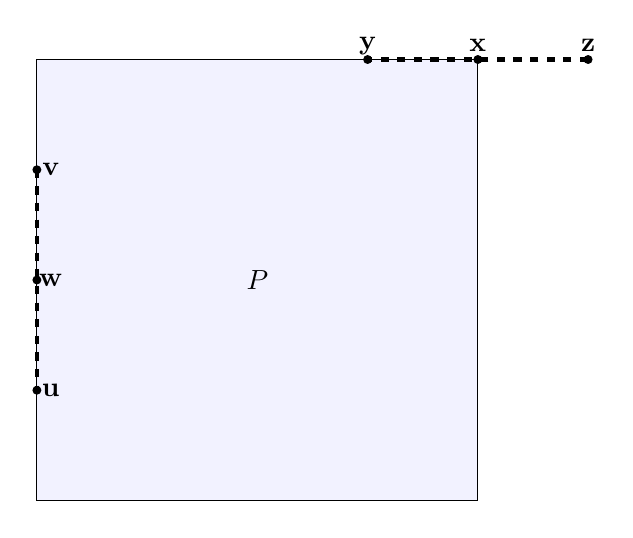
\begin{tikzpicture}[scale=0.7]
    \tikzset{punkt/.style={point, draw=black}}
    
    
%Punkter

	\node at (4,4)	(1){};
	\node at (-4,4)	(4){};
	\node at (4,-4)	(2){};
	\node at (-4,-4) (3){};


	\filldraw[black, fill=blue!5] (2) rectangle (4);
	\node at (0,0) (P){$P$};
	
	\filldraw [black] (2,4) circle (2pt);
	\filldraw [black] (4,4) circle (2pt);
	\filldraw [black] (6,4) circle (2pt);
	\filldraw [black] (-4,2) circle (2pt);
	\filldraw [black] (-4,0) circle (2pt);
	\filldraw [black] (-4,-2) circle (2pt);	
	\node at (2,4.25)	 (y){$\textbf{y}$};
	\node at (4,4.25)	 (x){$\textbf{x}$};
	\node at (6,4.25)	 (z){$\textbf{z}$};
	\node at (-3.75,2)  (v){$\textbf{v}$};
	\node at (-3.75,0)	 (w){$\textbf{w}$};
	\node at (-3.75,-2) (u){$\textbf{u}$};


	\draw[-, dashed,black,ultra thick] (6,4) -- (2,4);
	\draw[-, dashed,black,ultra thick] (-4,2) -- (-4,-2);

  \end{tikzpicture}
  \caption{En afgrænset polytop $P$ hvor $\textbf{x}$ er et ekstramapunkt da der ikke findes vektorer $\textbf{y}$ og $\textbf{z}$ sådan at $\mathbf{x}=\lambda\mathbf{y}+(1-\lambda)z$. $\textbf{w}$ er i modsætning ikke et ekstremapunkt da der findes $\textbf{v}$ og $\textbf{u}$ sådan at $\mathbf{w}=\lambda\mathbf{v}+(1-\lambda)u$.}
  \label{fig:ekstrema}
\end{figure}
%
%
%    \node[punkt] at (-4,0.5)      (v1){$v_1$};
%    \node[punkt] at (-2,0.5)      (v2){$v_2$};
%    \node[punkt] at (-4,-1.5)     (v3){$v_3$};
%    \node[punkt] at (-2,-1.5)     (v4){$v_4$};
%    \node at (-3,2)     (v){$K_{4}$};
%
%
%    \node[punkt] at (4.6,-0.2)      (k1){$v_3$};
%    \node[punkt] at (1.4,-0.2)      (k2){$v_2$};
%    \node[punkt] at (2,-2)     (k3){$v_4$};
%    \node[punkt] at (4,-2)     (k4){$v_5$};
%    \node[punkt] at (3,1)      (k5){$v_1$};
%    \node at (3,2)      (k){$K_{5}$};
%
%
%
%
%
%    \draw [-, thick, draw=black] (v1) -- (v2);
%    \draw [-, thick, draw=black] (v1) -- (v3);
%    \draw [-, thick, draw=black] (v1) -- (v4);
%    \draw [-, thick, draw=black] (v2) -- (v3);
%    \draw [-, thick, draw=black] (v2) -- (v4);
%    \draw [-, thick, draw=black] (v3) -- (v4);
\end{frame}
%
% Hjørnepunkt
%
\begin{frame}
\frametitle{Hjørner}
\begin{itemize}
\item Hjørnepunkter
\begin{itemize}
\item Alene i fællesmængde for $\mathcal{P}$ og hyperplan.
\end{itemize}
\end{itemize}
%
\input{Frames/4_mads/hjorne}
\end{frame}
%
% Basale mulige løsninger
%
\begin{frame}
\frametitle{Hjørner}
\begin{itemize}
\item Basale mulige løsninger
\begin{itemize}
\item Alle betingelser opfyldt og $n$ aktive betingelser
\end{itemize}
\end{itemize}
%
\begin{center}
%
\begin{tikzpicture}[scale=5]
%
% Koordinater
% -------------------------------------------------------
\coordinate (a) at (0,0,0); %tjek
\coordinate (b) at (0.7,0,0); % tjek
\coordinate (n) at (-0.15,0,0); % tjek
\coordinate (c) at (0.393,0.55,0); 
\coordinate (d) at (0.252,0.805,0);
\coordinate (e) at (0.066,0.434,0);
\coordinate (f) at (0,0.41,0);
\coordinate (g) at (0,0.305,0);
%
% Farvning
% -------------------------------------------------------
\filldraw[fill=myblue,opacity=0.3](a)--(b)--(c)--(e)--(g)--(a);
  \draw[thick](-0.2,-0.1,0)--(0.3,0.9,0); % n -> d  
  \draw[thick](0.2,0.9,0)--(0.757,-0.1,0); % d -> b
  \draw[thick](-0.3,0.3,0)--(0.8,0.7,0); % f -> c
  %\draw[thick](h)--(c);
% 
%
% Punkterne 
% -------------------------------------------------------
\filldraw [black] (b) circle (0.2pt) node[below] {$B$};
\filldraw [black] (a) circle (0.2pt) node[right] {$A$};
\filldraw [black] (n) circle (0.2pt) node[right] {$N$};
\filldraw [black] (c) circle (0.2pt) node[right] {$C$};
\filldraw [black] (d) circle (0.2pt) node[right] {$D$};
\filldraw [black] (e) circle (0.2pt) node[right] {$E$};
\filldraw [black] (f) circle (0.2pt) node[left] {$F$};
\filldraw [black] (g) circle (0.2pt) node[left] {$G$};
%
% Navngivning og prik til at gøre det pænt 
% -------------------------------------------------------
\draw[black] (0.91,0.96,1.2) circle (0pt) node[anchor=west] {$\mathcal{P}$};
\draw[black] (0,0,0.7) circle (0pt);
% 
% 
% Koordinatssystem 
% -------------------------------------------------------
\draw[thick,->] (0,0,0) -- (1,0,0) node[anchor=south east]{$x$};
\draw[thick] (0,0,0) -- (-0.2,0,0);
\draw[thick,->] (0,0,0) -- (0,1,0) node[anchor=north west]{$y$};
\draw[thick] (0,0,0) -- (0,-0.2,0);
%
\end{tikzpicture}
  \captionof{figure}{Punkterne $A,B,C,D,E,F$ og $G$ er basal løsninger, hvoraf $A,B,C,E$ og $F$ alle er basal mulige løsninger.}
  \label{fig:fig:basale}
\end{center}
%
\end{frame}
%
% Ækvivalens af hjørner
% (b) -> (a)
%
\begin{frame}
\frametitle{Ækvivalens mellem hjørner}
\begin{itemize}
\item Hjørnepunkt $\rightarrow$ ekstremumspunkt
\begin{itemize}
%
\item Hjørnepunkt giver
\end{itemize}
%
\centering
$
\begin{array}{ll}
\textbf{c}^T\textbf{u} < \textbf{c}^T\textbf{v}, &\textbf{v}\in \mathcal{P}, \textbf{v} \neq \textbf{u}\\
\textbf{c}^T\textbf{u} < \textbf{c}^T(\lambda\textbf{v} + (1-\lambda)\textbf{w}), &\textbf{v},\textbf{w} \in \mathcal{P}
\end{array}
$
%
\begin{itemize}
\item $\textbf{u}$ er ikke en konveks kombination
\end{itemize}
\end{itemize}
%
\end{frame}
%
% (a) -> (c)
%
\begin{frame}
\frametitle{Ækvivalens mellem hjørner}
\begin{itemize}
\item Ekstremumspunkt $\rightarrow$ basal mulig løsning
%
\begin{itemize}
\item Under $n$ aktive lineært uafhængige betingelser
\item $\textbf{d}$ ortogonal på underrummet
\item Lille $\varepsilon$
\end{itemize}

%
\centering
$
\begin{array}{ll}
\textbf{a}_i^T(\textbf{u} \pm \varepsilon \textbf{d}) > b_i, &i\notin I\\
\end{array}
$
\begin{itemize}
\item $\textbf{u}$ konveks kombination
\end{itemize}
\end{itemize}
%
\end{frame}
%
% (c) -> (b)
%
\begin{frame}
\frametitle{Ækvivalens mellem hjørner}
\begin{itemize}
\item Basal mulig løsning $\rightarrow$ hjørnepunkt
\begin{itemize}
\item Lav $\textbf{c} = \sum_{i\in I} \textbf{a}_i$
\end{itemize}
%
\begin{align*}
\textbf{c}^T\textbf{u} &= \sum_{i\in I} \textbf{a}_i^T\textbf{u} = 
 \sum_{i\in I} b_i\\
\textbf{c}^T\textbf{v} &= \sum_{i\in I} \textbf{a}_i^T\textbf{v} > 
 \sum_{i\in I} b_i, &\textbf{v}\in \mathcal{P}, \textbf{v} \neq \textbf{u}
\end{align*}
%
\begin{itemize}
\item $\textbf{u}$ alene i hyperplanet $\textbf{c}^T\textbf{x} = \sum_{i\in I} b_i$
\end{itemize}
\end{itemize}
\end{frame}
%
%
%
\begin{frame}
\frametitle{Løsning i hjørne}
\begin{itemize}
\item Mindst ét ekstremumspunkt og optimal løsning
\item $Q$ indeholder optimale løsninger i $\mathcal{P}$
\item $\textbf{u}$ optimale løsninger til $\mathcal{P}$ og ekstremumspunkt til $Q$
\item Antag $\textbf{u}$ ikke er ekstremumspunkt til $\mathcal{P}$
%
\begin{align*}
\textbf{u} &= \lambda\textbf{v} + (1-\lambda)\textbf{w}\\
\textbf{c}^T\textbf{v} &\geq y, \textbf{v} \in \mathcal{P}\\
\textbf{c}^T\textbf{v} &= \textbf{c}^T\textbf{w} = y
\end{align*}
%
\item $\textbf{u}$ ikke ekstremumspunkt i $Q$
%
\end{itemize}
\end{frame}